% sections/03-aspect-programming-overview.tex

\section{Aspect Programming Overview}
The core principle of the Aspect Programming framework is the Join Point Model (JPM). This model defines three key components:

\textbf{JoinPoint}: It specifies where the Aspect can run. A join point represents a specific point in the transaction processing flow and the block processing flow. It acts as a hook, allowing additional functional logic to be added at these points.

\textbf{Aspect}: It specifies the code to run on the join points. An Aspect can access the runtime context and make system calls, enabling it to participate in transaction lifecycle management.

\textbf{Binding}: It specifies when the Aspect can run. Smart contract owners have the freedom to bind Aspects to specific join points with their smart contracts. When transaction processing steps reach these join points, the bound Aspects are triggered.

\begin{figure}[htp]
  \centering
  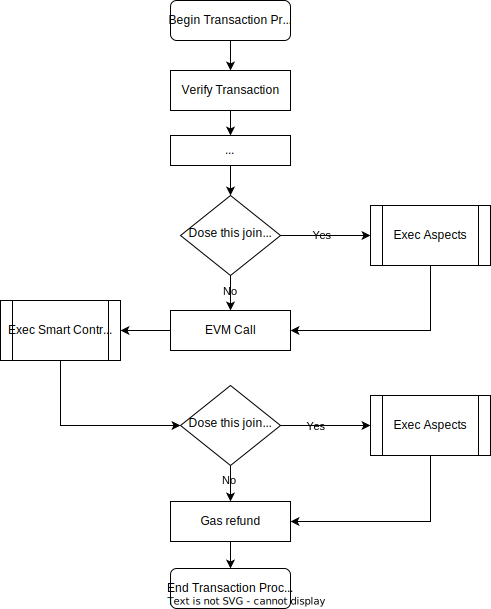
\includegraphics[width=0.5\textwidth]{sections/join-point-model-overview.png}
  \caption{Join Point Model}
\end{figure}

To provide a clearer understanding of how Aspect Programming works, let's walk through the transaction processes using an example. In this scenario, there is a smart contract with a vault function and a large deposit. The goal is to protect this smart contract at runtime to avoid illicit attacks that might illegally move out deposits. For this purpose, an Aspect is designed to be responsible for monitoring and verifying any deposit changes in the vault after smart contract execution. If there is an unexpected fund flow, the Aspect will revert the suspicious transaction. The Aspect execution is triggered after the smart contract execution when a transaction calls the smart contract.

\subsection{Aspect and Join Points}
An Aspect is implemented as a class that extends the Aspect base class. It contains methods that represent join points where additional logic can be injected. Here's an example implementation of an Aspect:

\begin{verbatim}
class SecurityAspect extends Aspect {
  @joinpoint
  postTxExecute(jpCtx: JPContext) {
    if (jpCtx.currentCall().methodName() == "withdraw") {
      let mintAmount = jpCtx.currentCall().params()[1];
      let actualVaultEtherFlow = jpCtx.stateChange(jpCtx.tx.to()).ether().diff();
      
      if (mintAmount != actualVaultEtherFlow) {
        jpCtx.txControl().revert();
      }
    }
  }
}
\end{verbatim}

In this example, the \texttt{postTxExecute} method serves as an entry point for the join point, which is triggered once the Ethereum Virtual Machine (EVM) completes transaction execution. The method is decorated with the \texttt{@joinpoint} annotation to indicate that it should be registered as a join point.

The \texttt{JPContext} object represents the runtime context and provides information about the original transaction, transaction runtime details at the current process point, and APIs for controlling transaction behavior. It is passed as a parameter to the join point method, enabling interaction with the transaction.

The example Aspect checks if the \texttt{withdraw} function of the smart contract is invoked during transaction execution. If so, it retrieves the expected minting amount from the transaction parameters and the actual funds flow of the vault from the runtime context. If there is a discrepancy between the expected and actual amounts, indicating a potential coding error or a cyberattack, the Aspect triggers the \texttt{revert()} function provided by the transaction management object in the runtime context, resulting in the reversal of the transaction.

\subsection{Deployment and Binding}
To deploy an Aspect onto the blockchain, its bytecode is included in a deployment transaction. This transaction calls an Aspect system contract, which stores the Aspect's bytecode within the blockchain's world state. Validators within the blockchain gain access to this bytecode, allowing them to execute the Aspect's logic when triggered.

However, an Aspect is only executed when it is bound to a specific smart contract. The binding process involves the smart contract owner signing a binding transaction using their externally owned account (EOA), the same account used for deploying the smart contract. This binding transaction includes the smart contract address and the Aspect ID. When this binding transaction is executed, it triggers the Aspect system contract, establishing the binding relationship between the smart contract and the Aspect within the blockchain's world state. Only the smart contract owner has the authority to bind Aspects to their smart contract, preventing unauthorized binding attempts by other EOAs.

Once the deployment and binding transactions are successfully processed, the Aspect is deployed onto the blockchain and bound to the smart contract. This integration enhances the capabilities and security of the smart contract by incorporating the Aspect's functionality.

\subsection{Execution with Aspect}
When a transaction is initiated on a smart contract, the Aspect Programming framework runtime is activated. As the transaction begins execution, the Aspect runtime evaluates each join point to determine if there are any bound Aspects associated with the invoked smart contract. If an Aspect is bound to a join point, it is triggered upon the completion of the transaction execution.

To execute an Aspect, the Aspect runtime retrieves its bytecode from the blockchain's world state and loads it into a WebAssembly (Wasm) runtime environment. A context object is then constructed, providing relevant information about the transaction and the execution environment. Finally, the Aspect runtime invokes the entry function of the Aspect, triggering the execution of the Aspect's logic.

For example, suppose the smart contract's \texttt{withdraw} function contains logic that ensures the transferred funds always exceed the amount specified in the function parameter. If an Aspect is bound to the \texttt{postTxExecute} join point, it will be triggered at the completion of the transaction execution. The Aspect runtime retrieves the Aspect's bytecode, loads it into the Wasm runtime, constructs a context object, and invokes the Aspect's entry function. If the Aspect identifies a discrepancy between the expected and actual funds transfer, it can set a revert flag via the join point context. Upon detecting this flag, the Aspect runtime reverses the transaction, labels the result as a failure, and provides a rationale specifying that the transaction was overturned by the bound Aspect.

\subsection{Conclusion}
The Aspect Programming framework's core component is the Join Point Model (JPM), which provides hooks for injecting additional logic at specific points in the transaction and block processing flows. Aspects, which contain the additional logic, can access the runtime context and make system calls to participate in transaction lifecycle management. By binding Aspects to specific join points, smart contract owners can enhance the capabilities and security of their contracts.

In the following sections, we will delve into a detailed design of the Join Point Model and its implementation.
